\documentclass[11pt,openany]{article}

\usepackage{mathtools, commath}
% Packages for formatting
\usepackage[margin=1in]{geometry}
\usepackage{fancyhdr}
\usepackage{enumerate}
\usepackage{graphicx}
\usepackage{kotex}
\usepackage{arydshln} % Include this package
\usepackage{bbding}
\usepackage{amsmath}
\usepackage{amsthm}
\usepackage[dvipsnames,table]{xcolor}
\usepackage{amssymb, amsfonts}
\usepackage{wasysym}
\usepackage{footnote}
\usepackage{tablefootnote}
\usepackage{arydshln} % Include this package
% Fonts
\usepackage[T1]{fontenc}
\usepackage[utf8]{inputenc}
\usepackage{newpxtext,newpxmath}
\usepackage{sectsty}

% Define colors
\definecolor{TealBlue1}{HTML}{0077c2}
\definecolor{TealBlue2}{HTML}{00a5e6}
\definecolor{TealBlue3}{HTML}{b3e0ff}
\definecolor{TealBlue4}{HTML}{00293c}
\definecolor{TealBlue5}{HTML}{e6f7ff}

\definecolor{thmcolor}{RGB}{231, 76, 60}
\definecolor{defcolor}{RGB}{52, 152, 219}
\definecolor{lemcolor}{RGB}{155, 89, 182}
\definecolor{corcolor}{RGB}{46, 204, 113}
\definecolor{procolor}{RGB}{241, 196, 15}

\usepackage{color,soul}
\usepackage{soul}
\newcommand{\mathcolorbox}[2]{\colorbox{#1}{$\displaystyle #2$}}
\usepackage{cancel}
\newcommand\crossout[3][black]{\renewcommand\CancelColor{\color{#1}}\cancelto{#2}{#3}}
\newcommand\ncrossout[2][black]{\renewcommand\CancelColor{\color{#1}}\cancel{#2}}

\usepackage{hyperref}
\usepackage{booktabs}

% Chapter formatting
\definecolor{titleTealBlue}{RGB}{0,53,128}
\usepackage{titlesec}
\titleformat{\section}
{\normalfont\sffamily\Large\bfseries\color{titleTealBlue!100!gray}}{\thesection}{1em}{}
\titleformat{\subsection}
{\normalfont\sffamily\large\bfseries\color{titleTealBlue!50!gray}}{\thesubsection}{1em}{}

%Tcolorbox
\usepackage[most]{tcolorbox}
\usepackage{multirow}
\usepackage{multicol}

\usepackage[linesnumbered,ruled]{algorithm2e}
\usepackage{algpseudocode}
\usepackage{setspace}
\SetKwComment{Comment}{/* }{ */}
\SetKwProg{Fn}{Function}{:}{end}
\SetKw{End}{end}
\SetKw{DownTo}{downto}

% Define a new environment for algorithms without line numbers
\newenvironment{algorithm2}[1][]{
	% Save the current state of the algorithm counter
	\newcounter{tempCounter}
	\setcounter{tempCounter}{\value{algocf}}
	% redefine the algorithm numbering (remove prefix)
	\renewcommand{\thealgocf}{}
	\begin{algorithm}
	}{
	\end{algorithm}
	% Restore the algorithm counter state
	\setcounter{algocf}{\value{tempCounter}}
}

\usepackage{adjustbox}
% Header and footer formatting
\pagestyle{fancy}
\fancyhead{}
\fancyhf{}
\rhead{\textcolor{TealBlue2}{\large\textbf{기대수(기초부터 대학원 수학까지 시리즈) 3기}}}%\rule{3cm}{0.4pt}}
\lhead{\textcolor{TealBlue2}{\large\textbf{수학의 즐거움, Enjoying Math}}}
% Define footer
%\newcommand{\footer}[1]{
%\begin{flushright}
%	\vspace{2em}
%	\includegraphics[width=2.5cm]{school_logo.jpg} \\
%	\vspace{1em}
%	\textcolor{TealBlue2}{\small\textbf{#1}}
%\end{flushright}
%}
%\rfoot{\large Department of Information Security, Cryptogrphy and Mathematics, Kookmin Uni.\includegraphics[height=1.5cm]{school_logo.jpg}}
\fancyfoot{}
\fancyfoot[C]{-\thepage-}

\usepackage{tcolorbox}
\tcbset{colback=white, arc=5pt}

\definecolor{axiomcolor}{HTML}{a88bfa}
\definecolor{defcolor}{RGB}{52, 152, 219}
\definecolor{procolor}{RGB}{241, 196, 15}
\definecolor{thmcolor}{RGB}{231, 76, 60}
\definecolor{lemcolor}{RGB}{155, 89, 182}
\definecolor{corcolor}{RGB}{46, 204, 113}
\definecolor{execolor}{RGB}{90, 128, 127}

% Define a new command for the custom tcolorbox
\newcommand{\axiombox}[2][]{%
	\begin{tcolorbox}[colframe=axiomcolor, title={\color{white}\bfseries #1}]
		#2
	\end{tcolorbox}
}

\newcommand{\defbox}[2][]{%
	\begin{tcolorbox}[colframe=defcolor, title={\color{white}\bfseries #1}]
		#2
	\end{tcolorbox}
}

\newcommand{\lembox}[2][]{%
	\begin{tcolorbox}[colframe=lemcolor, title={\color{white}\bfseries #1}]
		#2
	\end{tcolorbox}
}

\newcommand{\probox}[2][]{%
	\begin{tcolorbox}[colframe=procolor, title={\color{white}\bfseries #1}]
		#2
	\end{tcolorbox}
}

\newcommand{\thmbox}[2][]{%
	\begin{tcolorbox}[colframe=thmcolor, title={\color{white}\bfseries #1}]
		#2
	\end{tcolorbox}
}

\newcommand{\corbox}[2][]{%
	\begin{tcolorbox}[colframe=corcolor, title={\color{white}\bfseries #1}]
		#2
	\end{tcolorbox}
}



\usepackage{amsthm}

% Define custom theorem styles
\newtheoremstyle{dotless} % Name of the style
{3pt} % Space above
{3pt} % Space below
{\itshape} % Body font
{} % Indent amount
{\bfseries} % Theorem head font
{} % Punctuation after theorem head
{2.5mm} % Space after theorem head
{} % Theorem head spec

\newtheoremstyle{definitionstyle} % Name of the style
{3pt} % Space above
{3pt} % Space below
{} % Body font
{} % Indent amount
{\bfseries} % Theorem head font
{.} % Punctuation after theorem head
{2.5mm} % Space after theorem head
{} % Theorem head spec

% Applying custom styles
\theoremstyle{dotless}
\newtheorem{theorem}{Theorem} % Theorem environment with section-wise numbering
\newtheorem{proposition}[theorem]{Proposition} % Theorem environment with section-wise numbering
\newtheorem{lemma}[theorem]{Lemma} % Lemma shares the counter with theorem
\newtheorem{corollary}[theorem]{Corollary} % Corollary shares the counter with theorem

\theoremstyle{definitionstyle}
\newtheorem*{observation}{\textcolor{Magenta}{Observation}}
\newtheorem{definition}{Definition} % Definition shares the counter with theorem
\newtheorem{example}{Example} % Example shares the counter with theorem
\newtheorem{exercise}{Exercise} % Example shares the counter with theorem
\newtheorem{remark}{Remark} % Remark shares the counter with theorem
\newtheorem*{note}{Note}

\newtheorem*{definition*}{Definition} % Definition shares the counter with theorem
\newtheorem*{example*}{Example} % Example shares the counter with theorem
\newtheorem*{exercise*}{\textcolor{violet}{Exercise}} % Example shares the counter with theorem
\newtheorem*{remark*}{Remark} % Remark shares the counter with theorem


\usepackage{tikz}
\usepackage{tikz-cd}
\usepackage{tikz-3dplot}
\usepackage{pgfplots}
\pgfplotsset{compat=newest} % Adjust to your version of pgfplots
\def\Circlearrowleft{\ensuremath{%
		\rotatebox[origin=c]{180}{$\circlearrowleft$}}}
\def\Circlearrowright{\ensuremath{%
		\rotatebox[origin=c]{180}{$\circlearrowright$}}}
\def\CircleArrowleft{\ensuremath{%
		\reflectbox{\rotatebox[origin=c]{180}{$\circlearrowleft$}}}}
\def\CircleArrowright{\ensuremath{%
		\reflectbox{\rotatebox[origin=c]{180}{$\circlearrowright$}}}}
\usetikzlibrary{
	3d, % For 3D drawing
	angles,
	arrows,
	arrows.meta,
	backgrounds,
	bending,
	calc,
	decorations.pathmorphing,
	decorations.pathreplacing,
	decorations.markings,
	fit,
	matrix,
	patterns,
	patterns.meta,
	positioning,
	quotes,
	shadows,
	shapes,
	shapes.geometric,
	tikzmark
}
\tikzset{
	% single mid‐path arrow
	mid arrow/.style={
		decoration={
			markings,
			mark=at position 0.5 with {\arrow{Stealth[scale=1.2]}}
		},
		postaction={decorate},
	},
	% style for field arrows
	field arrow/.style={
		-{Stealth[scale=1.0]},
		thick,
		blue!70!black,
	},
}
\newcommand{\ie}{\textnormal{i.e.}}
\newcommand{\rsa}{\mathsf{RSA}}
\newcommand{\rsacrt}{\mathsf{RSA}\textendash\mathsf{CRT}}
\newcommand{\inv}[1]{#1^{-1}}

%New Command
%\newcommand{\set}[1]{\left\{#1\right\}}
\newcommand{\N}{\mathbb{N}}
\newcommand{\Z}{\mathbb{Z}}
\newcommand{\Q}{\mathbb{Q}}
\newcommand{\R}{\mathbb{R}}
\newcommand{\cR}{\mathcal{R}}
\newcommand{\C}{\mathbb{C}}
\newcommand{\F}{\mathbb{F}}
\newcommand{\nbhd}{\mathcal{N}}
\newcommand{\Log}{\operatorname{Log}}
\newcommand{\Arg}{\operatorname{Arg}}
\newcommand{\pv}{\operatorname{P.V.}}

\newcommand{\of}[1]{\left( #1 \right)} 
%\newcommand{\abs}[1]{\left\lvert #1 \right\rvert}
%\newcommand{\norm}[1]{\left\| #1 \right\|}

\newcommand{\sol}{\textcolor{magenta}{\bf Sol}}
\newcommand{\conjugate}[1]{\overline{#1}}

\newcommand{\res}{\operatorname{res}}
\DeclareMathOperator*{\Res}{\operatorname{Res}}

%\renewcommand{\Re}{\operatorname{Re}}
%\renewcommand{\Im}{\operatorname{Im}}

\newcommand{\cyclic}[1]{\langle #1 \rangle}
\newcommand{\uniform}{\overset{\$}{\leftarrow}}
\newcommand{\xmark}{\textcolor{red}{\XSolidBrush}}
\newcommand{\vmark}{\textcolor{green!75!black}{\CheckmarkBold}}

\newcommand{\gen}[1]{\langle #1 \rangle}
\newcommand{\Gen}[1]{\left\langle #1 \right\rangle}

\newcommand{\img}[1]{\text{Img}(#1)}
\newcommand{\Img}[1]{\text{Img}\left(#1\right)}
\newcommand{\preimg}[1]{\text{Img}^{-1}(#1)}
\newcommand{\Preimg}[1]{\text{Img}^{-1}\left(#1\right)}

\newcommand{\relation}{\mathrel{\mathcal{R}}}
\newcommand{\injection}{\rightarrowtail}
\newcommand{\surjection}{\twoheadrightarrow}
\newcommand{\id}{\textnormal{id}}

\newcommand{\eqclass}[1]{\left[#1\right]}

% Define custom colors for O and X
\newcommand{\yes}{\textcolor{blue}{\bf \fullmoon}}
\newcommand{\no}{\textcolor{red}{\bf \texttimes}}

\DeclarePairedDelimiter\ceil{\lceil}{\rceil}
\DeclarePairedDelimiter\floor{\lfloor}{\rfloor}
%\renewcommand{\floor}[#1]{\lfloor #1\rfloor}
%\newcommand{\Floor}[#1]{\left\lfloor #1\right\rfloor}
%\newcommand{\ceil}[#1]{\lceil #1\rceil}
%\newcommand{\Ceil}[#1]{\left\lceil #1\right\rceil}

\newcommand{\topology}{\mathscr{T}}
\newcommand{\sequence}[1]{\langle #1\rangle}

\setstretch{1.25}
\begin{document}
\pagenumbering{arabic}
\begin{center}
	\huge\textbf{Advanced Calculus II}\\
	\vspace{0.5em}
	\large{Ji, Yong-hyeon}\\
	\vspace{0.5em}
	\normalsize{\today}\\
\end{center}

\noindent 
We cover the following topics in this note.
\begin{itemize}
	\item Convergence of Sequences
	\item Inequality Rule for Absolute Values
	\item Limit Theorem (Algebraic Property of Limit of Sequence)
\end{itemize}
\hrule\vspace{12pt}
%Preliminaries:
%\begin{itemize}
%	\item Boundedness, Supremum and Infimum
%	\item Least Upper Bound Property (Completeness Axiom)
%	\item Well-Ordering Principle and Mathematical Induction
%	\item Archimedean Property
%\end{itemize}
%\hrule\vspace{12pt}

\vfill
\defbox[Sequence]{\begin{definition*}
	Let $X\subseteq\R$. A \textbf{sequence} is a function \[
	f:\N\to X(\subseteq\R),\quad n\mapsto f(n):=a_n.
	\] Instead of using function notation $f(n)$, the values of the sequence are denoted by $\set{a_n}_{n=1}^\infty$, where $a_n=f(n)$ is called $n$-th term of the sequence.
\end{definition*}}
\begin{remark*}
A sequence in $X\subseteq\R$ is a function \[
a:\N\to X,\quad n\mapsto a_n,
\] where $a_n\in X$ for all $n\in\N$. We sometimes write \[
\set{a_n},\quad\set{a_n}_{n=1}^\infty,\quad \set{a_n}_{n\in\N},\quad (a_n)_{n\in\N},\quad\ \text{or}\quad \gen{a_n}_{n\in\N}.
\]
\end{remark*}
\defbox[Convergence of Sequence]{\begin{definition*}
	A real sequence $\set{a_n}_{n=1}^\infty(\subseteq\R)$ is said to \textbf{converge} to $L\in\R$ if and only if \[
\forall\varepsilon>0,\ \exists N_\epsilon\in\N\ \text{such that}\ \left[ n\geq N_\epsilon\implies \abs{a_n-L}<\varepsilon\right].
\]	
\end{definition*}}
\begin{remark*}
	The real number $L\in\R$ is called \textbf{the limit}\footnote{The limit of a sequence is unique. See \hyperlink{thm4}{\textbf{Theorem 4}}}. When a sequence $\set{a_n}_{n=1}^\infty$ has the limit $L$, we will use the notation \[
	\lim_{n\to\infty}a_n=L\quad\text{or}\quad a_n\to L\ \text{as}\ n\to\infty.
	\]  That is, \[
		\lim_{n\to\infty}a_n=L\iff \forall\varepsilon>0:\exists N\in\N:\left[ n\geq N\implies \abs{a_n-L}<\varepsilon\right].
	\]
\end{remark*}
%\begin{remark*}
%		\\
%		&\iff\forall\varepsilon>0:\exists N(\varepsilon)\in\N:\left[ n\in[N(\varepsilon),\infty)\implies a(n)\in B_{\varepsilon}(L)\right] \\
%		&\iff \forall\varepsilon>0:\exists N(\varepsilon)\in\N:\left[ \set{a(n):n\in[N(\varepsilon),\infty)}\subseteq B_{\varepsilon}(L) \right]\\
%		&\iff\forall\varepsilon>0,\ \#\set{n\in\N: a_n\not\in(L-\varepsilon,L+\varepsilon)}<\infty.\\
%		&\iff \forall\varepsilon>0, a_n\in B_{\varepsilon}(L)\ \text{except some finite term.}
%	\end{align*}
%\end{remark*}

\newpage
\begin{note}
	If a sequence has a limit, we say that the sequence is \textbf{convergent}; if it has no limit, we say that the sequence is \textbf{divergent}.
\end{note}
\vfill
\begin{example*}
	Consider the sequence defined by $a_n=1/n$ for each $n\in\N$. Prove that \[
	\lim\limits_{n\to\infty}a_n=\lim\limits_{n\to\infty}\frac{1}{n}=0.
	\]
	\begin{center}
		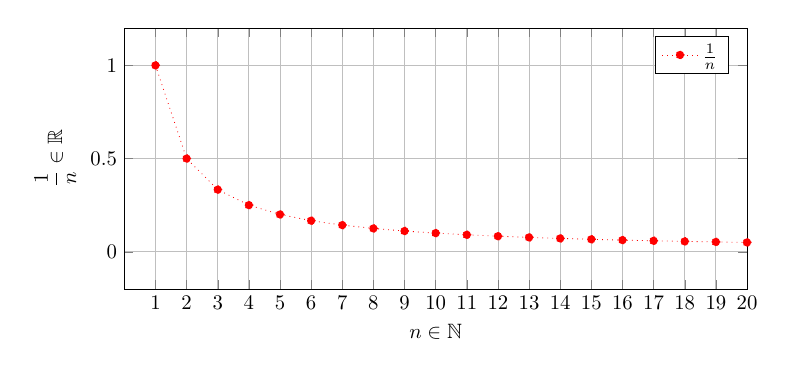
\begin{tikzpicture}[scale=.75]
	\begin{axis}[
		xlabel={$n \in \mathbb{N}$},
		ylabel={$\displaystyle\frac{1}{n}\in\R$},
		ymin=-.2, ymax=1.2,
		xmin=0, xmax=20,
		xtick={1,2,...,20},
		ytick={0,0.5,1},
		grid=major,
		width=\textwidth,
		height=6cm,
		domain=1:20,
		samples=20,
		legend pos=north east
		]
		% Plot points for 1 - 1/n
		%		\addplot[line width=.25mm, only marks, red, mark=x] plot (\x, 1 - 1/\x);
		\addplot[red, mark=*, dotted, mark options={fill=red}] plot (\x, 1/\x);
		\addlegendentry{$\frac{1}{n}$};
		
		% Draw horizontal line showing upper bound (y=1)
%		\addplot[dashed, magenta, line width=.5mm] coordinates {(0,1) (30,1)};
%		\node[magenta] at (axis cs: 3,1.1) {Upper Bound $1$};
		
		% Draw horizontal line showing lower bound (y=0)
%		\addplot[dashed, cyan, line width=.5mm] coordinates {(0,0) (30,0)};
%		\node[cyan] at (axis cs: 3,-0.1) {Lower Bound $0$};	
	\end{axis}
\end{tikzpicture}
	\end{center}
	\begin{proof}
		\textcolor{blue}{Let $\varepsilon>0$}. By the Archimedean property, we obtain \[
		\textcolor{blue}{\exists N_\epsilon\in\N}\quad \text{s.t.}\quad 1<\varepsilon\cdot N_\epsilon,\ \ie,\ \frac{1}{N_\epsilon}<\varepsilon.
		\] \textcolor{blue}{Assume that $n\geq N_\varepsilon$ then} \[
		\textcolor{blue}{\abs{a_n-0}}=\abs{\frac{1}{n}}=\frac{1}{n}\leq\frac{1}{N_\varepsilon}
		\textcolor{blue}{<\varepsilon}.
		\] Hence $\displaystyle\lim\limits_{n\to\infty}\frac{1}{n}=0$.
	\end{proof}
\end{example*}
\vfill
\begin{example*}
	Consider the sequence defined by $b_n=1-(-1)^n$ for all $n\in\N$. Prove that $b_n$ does not converge. 
	\begin{center}
		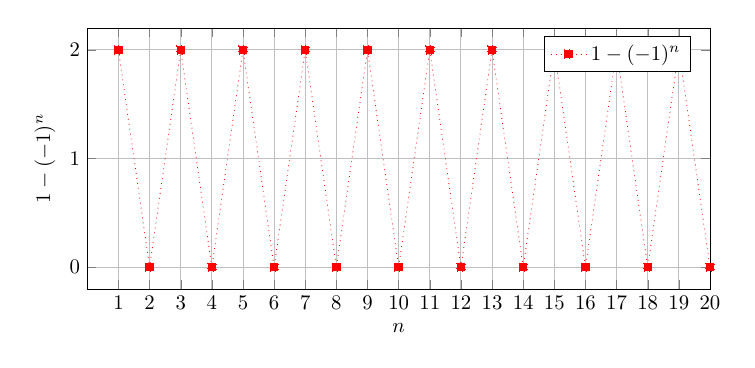
\begin{tikzpicture}[scale=.75]
	\begin{axis}[
		xlabel={$n$},
		ylabel={$1-(-1)^n$},
		ymin=-.2, ymax=2.2,
		xmin=0, xmax=20,
		xtick={1,2,...,20},
		ytick={0,1,2},
		grid=major,
		width=\textwidth,
		height=6cm,
		domain=1:20,
		samples=20,
		legend pos=north east,
		]
		\addplot[red, mark=square*, dotted, mark options={fill=red}] {1 - (-1)^x};
		\addlegendentry{$1-(-1)^n$};
		
		% Draw horizontal line showing upper bound (y=1)
		%		\addplot[dashed, magenta, line width=.5mm] coordinates {(0,1) (30,1)};
		%		\node[magenta] at (axis cs: 3,1.1) {Upper Bound $1$};
		
		% Draw horizontal line showing lower bound (y=0)
		%		\addplot[dashed, cyan, line width=.5mm] coordinates {(0,0) (30,0)};
		%		\node[cyan] at (axis cs: 3,-0.1) {Lower Bound $0$};	
	\end{axis}
\end{tikzpicture}
	\end{center}
	\begin{proof}
		The sequence $\set{b_n}$ alternates between $0$ and $2$: \[
		b_n=\begin{cases}
			0 &:n=2k \\
			2 &:n=2k+1
		\end{cases}
		\] with $k\in\N$.
		Suppose that $\set{b_n}_{n=1}^\infty$ converges to some limit $B\in\R$ and set
		$\varepsilon=1$. Then, by the definition of convergence:\[
		\exists N_\varepsilon\in\N\ \text{s.t.}\ n\geq N_\varepsilon\implies\abs{b_n-B}<1.
		\] \begin{enumerate}[(\text{Case} 1)]
			\item  For all even $n\geq N$, we have $b_n=0$.  Then the inequality $\abs{b_n-B}<1$ becomes \begin{equation}
				\abs{0-B}=\abs{B}<1,\ \ie, B\in(-1,1).
			\end{equation}
			\item For all odd $n\geq N$, we have $b_n=2$.  Then the inequality $\abs{b_n-B}<1$ becomes \begin{equation}
				\abs{2-B}<1,\ \ie,\ B\in\intoo{1,3}
			\end{equation}
		\end{enumerate}
		By (1) and (2), there is no intersection between these ranges; \[
		B\in(-1,1)\cap(1,3)=\varnothing
		\] which proves that $b_n$ does not converge.
		\begin{center}
			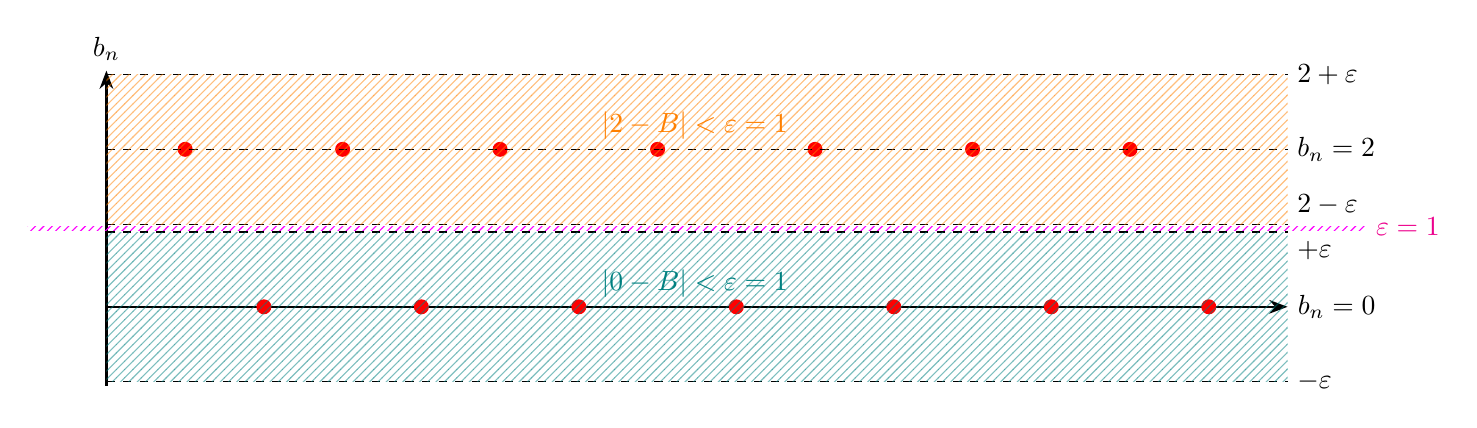
\begin{tikzpicture}[scale=1]
	% Define constants for visualization
	\def\B{2} % Hypothetical limit B
	\def\epsilon{.95} % Epsilon value
	\def\N{5} % Example N_epsilon value
	\def\xMax{15}
	\def\yMax{3} % Max value for y-axis
	\def\yMin{-1} % Min value for y-axis
	
	% Draw axes
	\draw[thick,-Stealth] (0,0) -- (\xMax,0) node[anchor=west] {$b_n=0$};
	\draw[thick,-Stealth] (0,\yMin) -- (0,\yMax) node[anchor=south] {$b_n$};
	
	% Draw limit B line and epsilon area
%	\draw[dashed] (0,\B) -- (10,\B) node[right] {$B$};
	\draw[dashed] (0,\B+\epsilon) -- (\xMax,\B+\epsilon) node[right] {$2+\varepsilon$};
	\draw[dashed] (0,\B-\epsilon) -- (\xMax,\B-\epsilon) node[above right] {$2-\varepsilon$};
	\draw[dashed] (0,+\epsilon) -- (\xMax,+\epsilon) node[below right] {$+\varepsilon$};
	\draw[dashed] (0,-\epsilon) -- (\xMax,-\epsilon) node[right] {$-\varepsilon$};
	
	% Sequence points
	\foreach \x in {1,...,14} {
		\pgfmathsetmacro{\parity}{mod(\x,2) == 0 ? 0 : 2}
		\filldraw[red] (\x,\parity) circle (2.5pt);
	}
	
	\draw[dashed] (0,2) to (\xMax, 2) node[right] {$b_n=2$};
	
	% Highlight issue area
	\fill[pattern=north east lines,pattern color=orange, opacity=.5] (0,\B+\epsilon) rectangle (\xMax,\B-\epsilon) node[midway, above, orange, opacity=1] {$\abs{2-B}<\varepsilon=1$};
	\fill[pattern=north east lines,pattern color=teal, opacity=.5] (0,-\epsilon) rectangle (\xMax,+\epsilon) node[midway, above, teal, opacity=1] {$\abs{0-B}<\varepsilon=1$};
	\fill[pattern=north east lines,pattern color=magenta] (-1,0.975) rectangle (\xMax+1,1.025) node[magenta, right] {$\varepsilon=1$};
	
	% Annotations to explain the issue
%	\node at (5,\B+\epsilon+0.5) [red] {Cannot cover $b_n=2$ when $n$ is odd};
%	\node at (5,\B-\epsilon-0.5) [blue] {Cannot cover $b_n=0$ when $n$ is even};
	
\end{tikzpicture}
		\end{center}
	\end{proof}
\end{example*}

%\begin{tikzpicture}[scale=1.5]
%	% Define constants for visualization
%	\def\N{5} % Example N_epsilon value
%	\def\yMax{3} % Max value for y-axis
%	\def\yMin{-1} % Min value for y-axis
%	
%	% Draw axes
%	\draw[thick,->] (0,0) -- (10,0) node[anchor=north] {$n$};
%	\draw[thick,->] (0,\yMin) -- (0,\yMax) node[anchor=east] {$b_n$};
%	
%	% Draw B regions
%	\draw[thick, blue] (0,1) -- (10,1) node[right] {$1$};
%	\draw[thick, blue] (0,-1) -- (10,-1) node[right] {$-1$};
%	\draw[thick, red] (0,3) -- (10,3) node[right] {$3$};
%	\draw[thick, red] (0,2) -- (10,2) node[right] {$2$};
%	
%	% Sequence points
%	\foreach \x in {1,...,9} {
%		\pgfmathsetmacro{\parity}{mod(\x,2) == 0 ? 0 : 2}
%		\filldraw (\x,\parity) circle (2pt);
%	}
%	
%	% Highlight the interval areas
%	\fill[blue, opacity=0.2] (0,-1) rectangle (10,1) node[pos=0.5, black, opacity=1] {$B \in (-1, 1)$};
%	\fill[red, opacity=0.2] (0,2) rectangle (10,3) node[pos=0.5, black, opacity=1] {$B \in (1, 3)$};
%	
%	% Annotations to explain the issue
%	\node at (5,0.5) [blue] {$B$ range for even $n$};
%	\node at (5,2.5) [red] {$B$ range for odd $n$};
%	\node at (5,\yMax) [black] {No intersection $\varnothing$};
%	
%\end{tikzpicture}
\newpage

\defbox[Absolute Value in Reals]{\begin{definition*}
	Let $x\in\R$. A \textbf{absolute value} $\abs{x}$ of $x$ is defined by \[
	\abs{x}:=\begin{cases}
		x &\text{if}\ x\geq 0\\
		-x &\text{if}\ x<0
	\end{cases}
	\]
\end{definition*}}
\begin{remark*}
	For $x\in\R$, \[
	\abs{x}=\begin{cases}
		x &:x>0 \\
		0 &:x=0\\
		-x &:x<0
	\end{cases}
	\]
\end{remark*}
\vfill
\probox[]{\begin{proposition}
Let $x,y\in\R$. \begin{enumerate}[\normalfont(1)]
	\item $\abs{x}=+\sqrt{x^2}$
	\item $\abs{x}\geq 0$
	\item $\abs{x}=0\Leftrightarrow x=0$
	\item $\abs{x}=\abs{-x}$
	\item $\abs{xy}=\abs{x}\abs{y}$
	\item (Fundamental Theorem of Absolute Values) For $c\geq 0$, we have \[
	\abs{x}\leq c\iff -c\leq x\leq c
	\]
	\item $-\abs{x}\leq x\leq\abs{x}$
\end{enumerate}
\end{proposition}}
\begin{proof}
\begin{enumerate}[(1)]
	\item If ($x\geq 0$) then $\abs{x}=x=\sqrt{x^2}$. Similarly if $x< 0$ then $\abs{x}=-x=\sqrt{x^2}$.
	\item $\abs{x}=\begin{cases}
		x\geq 0 &:x\geq 0\\
		-x>0 &:x<0
	\end{cases}\quad\geq 0$.
	\item[]
	\item \begin{itemize}
		\item[($\Leftarrow$)] If $x=0$ then $\abs{x}=x=0$.
		\item[($\Rightarrow$)] Let $\abs{x}=0$. Suppose that $x\neq0$. \begin{enumerate}[(i)]
			\item $x>0\implies \abs{x}=x>0\ \text{\Large\lightning}$
			\item $x<0\implies \abs{x}=-x>0\ \text{\Large\lightning}$
		\end{enumerate} Thus $x$ must be zero.
	\end{itemize}
	\newpage
	\item $\abs{-x}=\begin{cases}
		-x &: -x\geq 0\ (\ie, x\leq 0) \\
		-(-x)=x &: -x< 0\ (\ie, x> 0)
	\end{cases}=\begin{cases}
	x &\text{if}\ x\geq 0\\
	-x &\text{if}\ x<0
\end{cases}=\abs{x}$.
	\begin{center}
		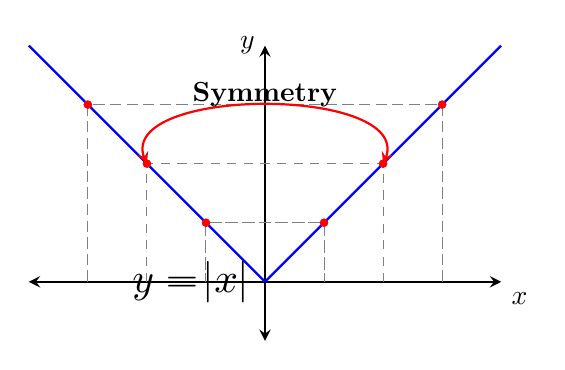
\begin{tikzpicture}[scale=1.5, >=stealth]
			% Draw axes
			\draw[<->, thick] (-2,0) -- (2,0) node[below right] {$x$};
			\draw[<->, thick] (0,-0.5) -- (0,2) node[left] {$y$};	
			% Plot |x|
			\draw[thick, domain=-2:0, samples=100, blue] plot (\x,{-\x}) node[pos=0.25, left, black] {$y = \abs{x}$};
			\draw[thick, domain=0:2, samples=100, blue] plot (\x,\x);
			% Mark points to illustrate symmetry
			\foreach \x in {-1.5, -1, -0.5, 0.5, 1, 1.5} {
				\draw[dashed, gray] (\x,0) -- (\x, {abs(\x)}) -- (-\x, {abs(\x)}) -- (-\x, 0);
				\fill[red] (\x, {abs(\x)}) circle (1pt);
				\fill[red] (-\x, {abs(\x)}) circle (1pt);
			}
			% Annotation for |x| = |-x|
%			\node at (1.5, 1.5) [above right, black] {$\abs{x} = \abs{-x}$};
%			\node at (-1.5, 1.5) [above left, black] {$\abs{x} = \abs{-x}$};
			% Symmetry arrows
			\draw[<->, thick, red] (1,1) to[out=60, in=120] (-1,1);
			\node[above] at (0,1.4) {\textbf{Symmetry}};
		\end{tikzpicture}
	\end{center}
	\item $\abs{xy}=\begin{cases}
		xy=\abs{x}\abs{y} &:x\geq0,y\geq 0\\
		-xy=x(-y)=\abs{x}\abs{y} &:x\geq0,y< 0\\
		-xy=(-x)y=\abs{x}\abs{y} &:x<0,y\geq 0\\
		xy=(-x)(-y)=\abs{x}\abs{y} &:x<0,y< 0
	\end{cases}$
%	\begin{center}
%	\begin{tikzpicture}
%		\begin{axis}[
%			width=12cm,
%			view={15}{45}, % 3D view angles
%			axis lines=center,
%			xlabel={$x$},
%			ylabel={$y$},
%			zlabel={$z$},
%			xtick={-5,-4,-3,-2,-1,0,1,2,3,4,5},
%			ytick={-5,-4,-3,-2,-1,0,1,2,3,4,5},
%			ztick={-5,-4,-3,-2,-1,0,1,2,3,4,5},
%			domain=-10:10,
%			samples=50,
%			samples y=50,
%			colormap/viridis,
%			zmax=10,
%			zmin=0
%			]
%%			% Plot z = xy
%%			\addplot3[surf, opacity=0.5, mesh, domain=-2:2, samples=30, samples y=30] 
%%			{x * y};
%%			\addlegendentry{$z = xy$};
%			
%			% Plot z = |xy|
%%			\addplot3[surf, opacity=0.7, colormap/hot, domain=-5:5, samples=50, samples y=50] 
%%			{abs(x * y)};
%%			\addlegendentry{$z = \abs{xy}$};
%			\addplot3[surf, opacity=0.7, mesh, domain=-6:6, samples=50, samples y=50] 
%			{abs(x * y)};
%			\addlegendentry{$z = \abs{xy}$};
%			
%		\end{axis}
%	\end{tikzpicture}
%	\end{center}
	\vspace{1cm}
	\item[\textcolor{red}{(6)}] 
	\begin{itemize}
		\item[($\Rightarrow$)] Let $\abs{x}\leq c$. \begin{enumerate}[(i)]
			\item $x\geq 0\implies x=\abs{x}\leq c$, \ie, $-c\leq 0\leq x\leq c$.
			\item $x<0\implies -x=\abs{x}\leq c$, \ie, $-c\leq x< 0\leq c$.
		\end{enumerate} Thus, $-c\leq x\leq c$.
		\vspace{.5cm}
		\item[($\Leftarrow$)] Let $-c\leq x\leq c$. \begin{enumerate}[(i)]
			\item $x\geq 0\implies \abs{x}=x\leq c$.
			\item $x<0\implies \abs{x}=-x\leq c$.
		\end{enumerate} Thus, $\abs{x}\leq c$.
	\end{itemize}
	\begin{center}
	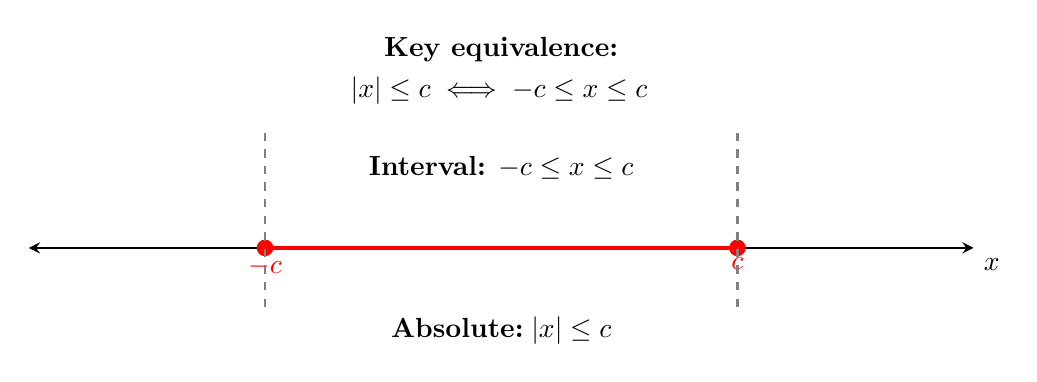
\begin{tikzpicture}[scale=1.5, >=stealth]
		
		% Number line
		\draw[<->, thick] (-4,0) -- (4,0) node[below right] {$x$};
		
		% Points and labels for -c, c
		\fill[red] (-2,0) circle (2pt) node[below] {$-c$};
		\fill[red] (2,0) circle (2pt) node[below] {$c$};
		
		% Shading for interval -c to c
		\draw[red, ultra thick] (-2,0) -- (2,0);
		
		% Dashes to show bounds
		\draw[dashed, thick, gray] (-2,-0.5) -- (-2,1) node[above, black] {};
		\draw[dashed, thick, gray] (2,-0.5) -- (2,1);
		
		% Annotation for interval
		\node[above] at (0, 0.5) {\textbf{Interval:} $-c \leq x \leq c$};
		\node[below] at (0, -0.5) {\textbf{Absolute:} $\abs{x} \leq c$};
		
		% Equivalence explanation
		\node at (0, 1.5) [align=center, black] 
		{\textbf{Key equivalence:} \\[3pt] 
			$\abs{x} \leq c \iff -c \leq x \leq c$};
	\end{tikzpicture}
\end{center}
	\item[(7)] Let $c=\abs{x}$, where $c\geq 0$. By (6), thus, the result follows.
\end{enumerate}
\end{proof}
\vfill
\probox[Triangle Inequality]{\begin{proposition}
Let $x,y\in\R$. \begin{enumerate}[\normalfont(1)]
	\item $\abs{x+y}\leq\abs{x}+\abs{y}$
	\item $\abs{\abs{x}-\abs{y}}\leq\abs{x-y}$.
\end{enumerate}
\end{proposition}}
\begin{center}
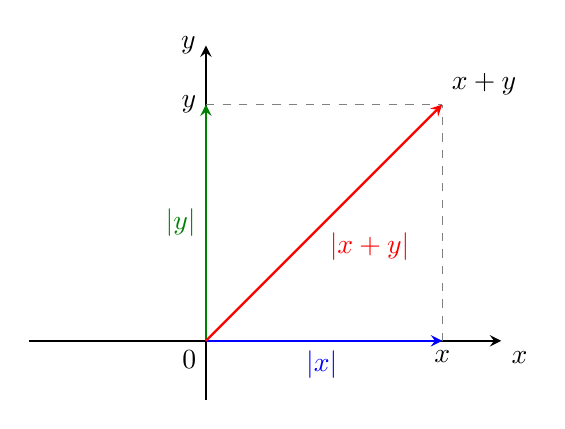
\begin{tikzpicture}[scale=1.5, >=stealth]
	
	% Axes
	\draw[->, thick] (-1.5,0) -- (2.5,0) node[below right] {$x$};
	\draw[->, thick] (0,-0.5) -- (0,2.5) node[left] {$y$};
	
	% Points
	\coordinate (A) at (0,0); % Origin
	\coordinate (B) at (2,0); % x
	\coordinate (C) at (0,2); % y
	\coordinate (D) at (2,2); % x+y
	
	% Vectors
	\draw[thick, blue, ->] (A) -- (B) node[midway, below] {$\abs{x}$};
	\draw[thick, green!50!black, ->] (A) -- (C) node[midway, left] {$\abs{y}$};
	\draw[thick, red, ->] (A) -- (D) node[midway, below right] {$\abs{x + y}$};
	
	% Dashed lines to form triangle
	\draw[dashed, gray] (B) -- (D);
	\draw[dashed, gray] (C) -- (D);
	
	% Labels for points
	\node[below left] at (A) {$0$};
	\node[below] at (B) {$x$};
	\node[left] at (C) {$y$};
	\node[above right] at (D) {$x + y$};
	
	% Inequality explanation
%	\node[align=center] at (1, 2.5) 
%	{\textbf{Triangle Inequality:} \\[3pt] 
%		$\abs{x + y} \leq \abs{x} + \abs{y}$ \\[3pt]
%		\textit{(Red vector is shorter than or equal to the sum of blue and green vectors)}};
\end{tikzpicture}
\end{center}
\begin{proof}
\begin{enumerate}[(1)]
	\item By (7) of \textbf{Proposition 1}, we have \[
	-\abs{x}\leq x\leq\abs{x},\quad-\abs{y}\leq y\leq\abs{y}.
	\]
	Then \begin{table}[h!]\centering\setstretch{1.5}
		\begin{tabular}{cccccc}
			&$-\abs{x}$ & $\leq$ & $x$ & $\leq$ & $\abs{x}$ \\
			+&$-\abs{y}$ & $\leq$ & $y$ & $\leq$ & $\abs{y}$ \\ \cline{2-6}
			&$-(\abs{x}+\abs{y})$& $\leq$& $x+y$&$\leq$& $\abs{x}+\abs{y}$ \\
		\end{tabular}
	\end{table}\\ Thus, we have $\abs{x+y}\leq\abs{x}+\abs{y}$.
	\item \ \begin{enumerate}[(i)]
		\item Note that \begin{align*}
			\abs{x} &=\abs{x-y+y} \\
			&\leq\abs{x-y}+\abs{y}\quad\text{by (1) of \textbf{Proposition 2}}
		\end{align*} Thus $\abs{x}-\abs{y}\leq\abs{x-y}$. 
		\item Note that \begin{align*}
			\abs{y}&=\abs{x-(x-y)}\\
			&\leq\abs{x}+\abs{-(x-y)}\quad\text{by (1) of \textbf{Proposition 2}} \\
			&=\abs{x}+\abs{x-y}\quad\text{by (4) of \textbf{Proposition 1}}
		\end{align*} Therefore $-\abs{x-y}\leq\abs{x}-\abs{y}$.
	\end{enumerate} By (i) and (ii), we know \[
	-\abs{x-y}\leq\abs{x}-\abs{y}\leq\abs{x-y},\quad\ie,\quad\abs{\abs{x}-\abs{y}}\leq\abs{x-y}.
	\]
\end{enumerate}
\end{proof}
\vfill
\defbox[Boundedness of Sequence]{\begin{definition*}
	Let $\set{a_n}_{n=1}^\infty(\subseteq\R)$ is a sequence. $\set{a_n}$ is said to be \textbf{bounded} if \[
		\exists M\in\R\ \text{such that}\ \forall n\in\N,\ \abs{a_n}\leq M.
		\]
\end{definition*}}
\vfill
\probox[]{\begin{proposition}\hypertarget{pro3}{}
	A convergent sequence is bounded.
\end{proposition}}
\begin{proof}
	Let $\lim\limits_{n\to\infty}a_n=L$. By the definition of convergence, for $\varepsilon=1$,  \[
	\exists N\in\N\ \text{such that}\ n\geq N\implies\abs{a_n-L}<1.
	\] By triangle inequality, we have \[
	\abs{a_n}=\abs{a_n-L+L}\leq\abs{a_n-L}+\abs{L}<1+\abs{L}.
	\] Let $M:=\max\set{\abs{a_1},\abs{a_2},\dots,\abs{a_{N-1}},1+\abs{L}}$. Then \[
	\abs{a_n}\leq M
	\] for all $n\in\N$. Therefore $\set{a_n}$ is bounded.
\begin{center}
	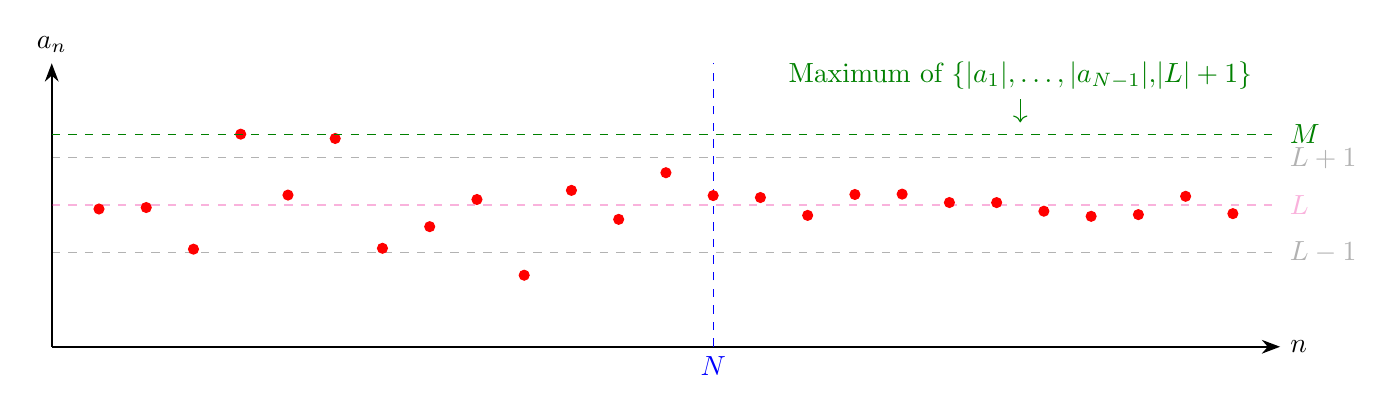
\begin{tikzpicture}[scale=.6]
	% Define the coordinates for L and the bounding lines
	\def\L{3} % Set L at 3 for visualization
	\def\epsilon{1} % Epsilon value
	\def\N{14} % Example N value
	\def\xMax{25}
	\def\yMax{6} % Max value for y-axis
	
	% Draw axes
	\draw[thick,-Stealth] (0,0) -- (\xMax+1,0) node[anchor=west] {$n$};
	\draw[thick,-Stealth] (0,0) -- (0,\yMax) node[anchor=south] {$a_n$};
	
	% Draw L and epsilon lines
	\draw[dashed, magenta, opacity=.3] (0,\L) -- (\xMax+1,\L) node[right] {$L$};
	\draw[dashed, opacity=.3] (0,\L+\epsilon) -- (\xMax+1,\L+\epsilon) node[right] {$L+1$};
	\draw[dashed, opacity=.3] (0,\L-\epsilon) -- (\xMax+1,\L-\epsilon) node[right] {$L-1$};
	
	% Mark the N line
	\draw[dashed, blue] (\N,0) -- (\N,\yMax) node[at start, below] {$N$};
	
	% Points of a_n for n < N and n >= N
	\foreach \x in {1,2,3,5,6,...,13} {
		\pgfmathsetmacro{\y}{rand*1.5+\L}
		\filldraw[red] (\x,\y) circle (3pt);
	}
	\filldraw[red] (4,4.5) circle (3pt);
	\foreach \x in {\N,...,\xMax} {
		\pgfmathsetmacro{\y}{rand*0.25+\L}
		\filldraw[red] (\x,\y) circle (3pt);
	}
	
	% Draw M line
	\def\M{4.5} % example M value
	\draw[dashed, green!50!black] (0,\M) -- (\xMax+1,\M) node[right] {$M$};
	
	% Labeling M
	\draw[<-, green!50!black] (20.5,4.75) -- (20.5,5.25) node[above] {Maximum of $\{\lvert a_1 \rvert, \dots, \lvert a_{N-1} \rvert, \abs{L}+1\}$};
\end{tikzpicture}
\end{center}
\end{proof}
\vfill
\begin{note}
	We have established that if the limit of a sequence \(a_n\) exists as \(n\) approaches infinity, then there exists a real number \(M\) such that \(\lvert a_n \rvert \leq M\) for all \(n\): \[
	\exists A\in\R\ \text{s.t.}\ A=\lim_{n\to\infty}a_n\implies\exists M\in\R\ \text{s.t.}\ \forall n\in\N,\ \abs{a_n}\leq M.
	\]However, the converse is not necessarily true: \[
	\exists A\in\R\ \text{s.t.}\ A=\lim_{n\to\infty}a_n\centernot\impliedby\exists M\in\R\ \text{s.t.}\ \forall n\in\N,\ \abs{a_n}\leq M.
	\] To illustrate, consider the sequence \(\{a_n\} = 1 - (-1)^n\). This sequence is bounded, yet it does not converge, serving as a counterexample.
	\vfill
	\noindent Furthermore, we note the following important theorems:
	\begin{enumerate}
		\item \textbf{Monotone Convergence Theorem}:
		\begin{enumerate}[(i)]
			\item If a sequence \(\{a_n\}\) is bounded above and monotone increasing, then it converges.
			\item If a sequence \(\{a_n\}\) is bounded below and monotone decreasing, then it converges.
		\end{enumerate}
		\item \textbf{Bolzano-Weierstrass Theorem}: Every bounded sequence of real numbers has a convergent subsequence. That is, if there exists a real number \(M\) such that \(\lvert a_n \rvert < M\) for all \(n\), then there exists a convergent subsequence \(\{a_{n_k}\}\) of \(\{a_n\}\).
	\end{enumerate}
\end{note}

%\begin{tikzpicture}[scale=2]
%	\begin{axis}[
%		title=Example using the mesh parameter,
%		hide axis,
%		colormap/cool,
%		]
%		\addplot3[
%		mesh,
%		samples=50,
%		domain=-8:8,
%		]
%		{sin(deg(sqrt(x^2+y^2)))/sqrt(x^2+y^2)};
%		\addlegendentry{\(\frac{sin(r)}{r}\)}
%	\end{axis}
%\end{tikzpicture}
%\newpage
\vfill
\thmbox[Limit Theorem (Algebraic Property of Limit of Sequence)]{
\begin{theorem*} Let $\lim\limits_{n\to\infty}a_n=\alpha$, $\lim\limits_{n\to\infty}b_n=\beta$, and $k\in\R$. Then 
\begin{enumerate}[(1)]
	\item $\lim\limits_{n\to\infty}k a_n=k\alpha=k\lim\limits_{n\to\infty}a_n$.
	\item $\lim\limits_{n\to\infty}a_n\pm b_n=\alpha\pm\beta=\lim\limits_{n\to\infty}a_n\pm\lim\limits_{n\to\infty}b_n$.
	\item $\lim\limits_{n\to\infty}a_n b_n=\alpha\beta=\lim\limits_{n\to\infty}a_n\lim\limits_{n\to\infty}b_n$.
	\item $\displaystyle\lim\limits_{n\to\infty}\frac{a_n}{b_n}=\frac{\alpha}{\beta}=\frac{\lim\limits_{n\to\infty}a_n}{\lim\limits_{n\to\infty}b_n}$. \normalfont (Here, $\beta\neq 0$ and $b_n\neq 0$)
%	\item $\lim\limits_{n\to\infty}\abs{a_n}=\abs{\lim\limits_{n\to\infty}a_n}=\abs{A}$.
%	\item $\lim\limits_{n\to\infty}(a_n)^p=A^p$. (Here, $p\in\N$).
%	\item $[\exists K:n\geq K\implies a_n\leq b_n]\implies A\leq B$.
\end{enumerate}
\end{theorem*}}
\begin{proof}
\textcolor{blue}{Let $\varepsilon>0$}. \begin{enumerate}[(1)]
	\item If $k=0$, it is trivial. Let $k\neq 0$. Since $\lim\limits_{n\to\infty}a_n=\alpha$, we know \[
	\textcolor{blue}{\exists N\in\N}\ \text{such that}\ \left[n\geq N\implies\abs{a_n-\alpha}<\textcolor{red}{\frac{\varepsilon}{\abs{k}}}\right]\label{eq:eq1} \tag{*}
	\] Thus, \textcolor{blue}{if $n\geq N$ then} \begin{align*}
	\textcolor{blue}{\abs{ka_n-k\alpha}}&=\abs{k(a_n-\alpha)}\\
	&=\abs{k}\abs{a_n-\alpha}\quad\because \abs{xy}=\abs{x}\abs{y}\\
	&\textcolor{blue}{<}\abs{k}\cdot\textcolor{red}{\frac{\varepsilon}{\abs{k}}}\quad\text{by (*)}\\
	&=\textcolor{blue}{\varepsilon}.
	\end{align*}
	\begin{center}
	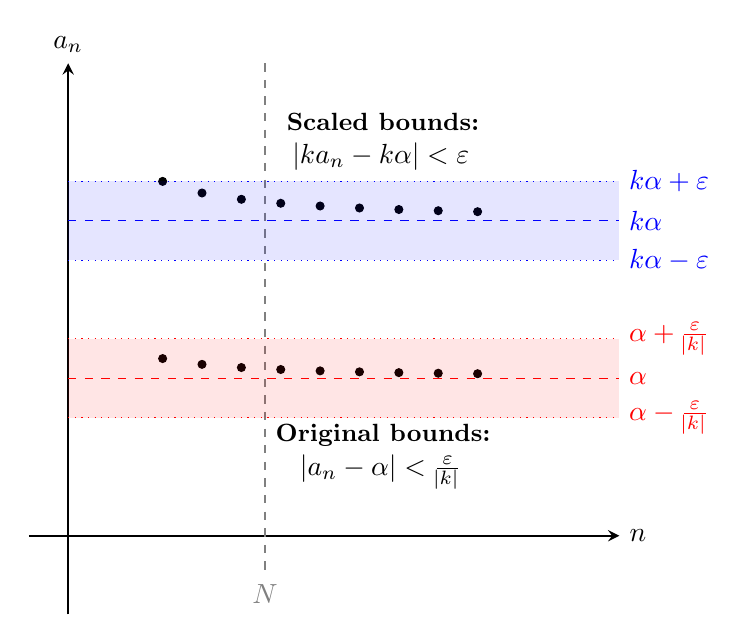
\begin{tikzpicture}[scale=1, >=stealth]
		
		% Axes
		\draw[->, thick] (-0.5, 0) -- (7, 0) node[right] {$n$};
		\draw[->, thick] (0, -1) -- (0, 6) node[above] {$a_n$};
		
		% Original limit A
		\draw[dashed, red] (0, 2) -- (7, 2) node[right] {$\alpha$};
		
		% Scaled limit alpha A
		\draw[dashed, blue] (0, 4) -- (7, 4) node[right] {$k\alpha$};
		
		% Epsilon bounds around A
		\draw[dotted, red] (0, 2.5) -- (7, 2.5) node[right] {$\alpha + \frac{\varepsilon}{\abs{k}}$};
		\draw[dotted, red] (0, 1.5) -- (7, 1.5) node[right] {$\alpha - \frac{\varepsilon}{\abs{k}}$};
		
		% Epsilon bounds around alpha A
		\draw[dotted, blue] (0, 4.5) -- (7, 4.5) node[right] {$k\alpha + \varepsilon$};
		\draw[dotted, blue] (0, 3.5) -- (7, 3.5) node[right] {$k\alpha - \varepsilon$};
		
		% Sequence points a_n
		\foreach \x in {1.2, 1.7, 2.2, 2.7, 3.2, 3.7, 4.2, 4.7, 5.2} {
			\draw[fill=black] (\x, {2 + (0.3 / \x)}) circle (0.05); % Points near A
		}
		
		% Sequence points alpha a_n
		\foreach \x in {1.2, 1.7, 2.2, 2.7, 3.2, 3.7, 4.2, 4.7, 5.2} {
			\draw[fill=black] (\x, {4 + (0.6 / \x)}) circle (0.05); % Points near alpha A
		}
		
		% N marker
		\draw[dashed, gray] (2.5, 6) -- (2.5, -0.5) node[below] {$N$};
%		\node[below] at (2.5, -0.5) {$n = N$};
		
		% Overlap annotation for scaled sequence
		\fill[blue, opacity=0.1] (0, 3.5) rectangle (7, 4.5);
		\node[align=center] at (4, 5) {\textbf{\small Scaled bounds:} \\ $\abs{ka_n - k\alpha} < \varepsilon$};
		
		% Original bounds annotation
		\fill[red, opacity=0.1] (0, 1.5) rectangle (7, 2.5);
		\node[align=center] at (4, 1) {\textbf{\small Original bounds:} \\ $\abs{a_n - \alpha} < \frac{\varepsilon}{\abs{k}}$};
		
		% Explanation of scaling
%		\node[align=center] at (4, -0.8) 
%		{\textbf{Scaling property:} \\[5pt] 
%			$\abs{\alpha a_n - \alpha A} = \abs{\alpha} \abs{a_n - A}$.};
	\end{tikzpicture}
	\end{center}
	\item Since $\lim\limits_{n\to\infty}a_n=\alpha$ and $\lim\limits_{n\to\infty}b_n=\beta$, we know that \begin{align*}
		\exists N_1\in\N\ \text{such that}\ \left[n\geq N_1\implies\abs{a_n-\alpha}<\textcolor{red}{\frac{\varepsilon}{2}}\right]\label{eq:eq2} \tag{**}\\
		\exists N_2\in\N\ \text{such that}\ \left[n\geq N_2\implies\abs{b_n-\beta}<\textcolor{red}{\frac{\varepsilon}{2}}\right]\label{eq:eq3} \tag{***}
	\end{align*} Let $\textcolor{blue}{N=\max\set{N_1,N_2}}$. \textcolor{blue}{If $n\geq N$ then} \begin{align*}
	\textcolor{blue}{\abs{(a_n+ b_n)-(\alpha+ \beta)}}&=\abs{(a_n-\alpha)+(b_n-\beta)}\\
	&\leq\abs{a_n-\alpha}+\abs{b_n-\beta}\quad\text{by Triangle Inequality}\\
	&\textcolor{blue}{<}\textcolor{red}{\frac{\varepsilon}{2}}+\textcolor{red}{\frac{\varepsilon}{2}}\quad\text{by (**) and (***)}\\
	&=\textcolor{blue}{\varepsilon}.
\end{align*} and \[
	\textcolor{blue}{\abs{(a_n- b_n)-(\alpha- \beta)}}=\abs{(a_n-\alpha)+(-b_n+\beta)}\leq\abs{a_n-\alpha}+\abs{b_n-\beta}\textcolor{blue}{<}\textcolor{red}{\frac{\varepsilon}{2}}+\textcolor{red}{\frac{\varepsilon}{2}}=\textcolor{blue}{\varepsilon}.
	\]
	\vfill
	\item  By \hyperlink{pro3}{\textbf{Proposition 3}}, $\set{a_n}$ is bounded and so \[
	\exists M>0\ \text{such that}\ \forall n\in N,\ \abs{a_n}\leq M.
	\] Note that \begin{align*}
		\lim\limits_{n\to\infty}a_n=\alpha\implies\exists N_1\in\N:&\left[n\geq N_1\implies\abs{a_n-\alpha}<\textcolor{red}{\frac{\varepsilon}{2\abs{\beta}+1}}\right],\\ \lim\limits_{n\to\infty}b_n=\beta\implies\exists N_2\in\N:&\left[n\geq N_2\implies\abs{b_n-\beta}<\textcolor{red}{\frac{\varepsilon}{2M}}\right].
	\end{align*} Let $\textcolor{blue}{N=\max\set{N_1,N_2}}$. \textcolor{blue}{If $n\geq N$ then} \begin{align*}
		\textcolor{blue}{\abs{a_nb_n-\alpha\beta}}=\abs{a_nb_n-\alpha\beta\ \textcolor{green!50!black}{+\ a_n\beta\ -\ a_n\beta}}&=\abs{a_n(b_n-\beta)+\beta(a_n-\alpha)}\\
		&\leq\abs{a_n}\abs{b_n-\beta}+\abs{\beta}\abs{a_n-\alpha}\\
		&<M\cdot\textcolor{red}{\frac{\varepsilon}{2M}}+\textcolor{red}{\frac{\abs{\beta}}{2\abs{\beta}+1}}\cdot\varepsilon\\
		&\textcolor{blue}{<}\frac{\varepsilon}{2}+\frac{\varepsilon}{2}=\textcolor{blue}{\varepsilon}.
	\end{align*} \textcolor{gray!50}{Note that $2\abs{\beta}<2\abs{\beta}+1\Leftrightarrow\frac{\abs{\beta}}{2\abs{\beta}+1}<\frac{1}{2}$.}
	\item It is enough to prove that $\displaystyle\lim\limits_{n\to\infty}\frac{1}{b_n}=\frac{1}{\beta}$ with $b_n\neq 0$ and $\beta\neq 0$. Note that Triangle Inequality implies that \[
	\abs{y}=\abs{y-x+x}\leq\abs{y-x}+\abs{x}\iff\abs{y}-\abs{x}\leq\abs{y-x}
	\] for any $x,y\in\R$. Since $\lim\limits_{n\to\infty}b_n=\beta$, for $\displaystyle\textcolor{red}{\frac{1}{2}\abs{\beta}}\textcolor{blue}{>0}$, $\exists N_1\in\N$ such that if $n\geq N_1$ \[
	\abs{\beta}-\abs{b_n}\leq\abs{\beta-b_n}=\abs{b_n-\beta}<\textcolor{red}{\frac{1}{2}\abs{\beta}}.
	\] Thus, we obtain that \[
	\abs{\beta}-\abs{b_n}<\frac{1}{2}\abs{\beta}\implies\frac{1}{2}\abs{\beta}<\abs{b_n}\implies\textcolor{teal}{\frac{1}{b_n}<\frac{2}{\abs{\beta}}}
	\] And \[
	\exists N_2\in\N:\left[n\geq N_2\implies\textcolor{orange}{\abs{b_n-\beta}<\frac{\beta^2}{2}\varepsilon}\right].
	\] Let \textcolor{blue}{$N=\max\set{N_1,N_2}$}. \textcolor{blue}{If $n\geq N$ then} \[
	\textcolor{blue}{\abs{\frac{1}{b_n}-\frac{1}{\beta}}}=\abs{\frac{\beta-b_n}{\beta b_n}}=\frac{\textcolor{orange}{\abs{b_n-\beta}}}{\abs{\beta}\textcolor{teal}{\abs{b_n}}}\textcolor{blue}{<}\textcolor{orange}{\varepsilon\cdot\frac{\beta^2}{2}}\cdot\frac{1}{\abs{\beta}}\textcolor{teal}{\cdot\frac{2}{\abs{\beta}}}=\textcolor{blue}{\varepsilon}.
	\]
\end{enumerate}
\end{proof}
\thmbox[Uniqueness of Limits]{\begin{theorem}\hypertarget{thm4}{}
	The limit of a sequence is unique.
\end{theorem}}
\begin{proof}
We want to show that \[
\lim\limits_{n\to\infty}a_n=\alpha\ \text{and}\ \lim\limits_{n\to\infty}a_n=\beta\implies\alpha=\beta.
\] Let a sequence $\set{a_n}$ has limit $\alpha$ and $\beta$, and \textcolor{blue}{let $\varepsilon>0$}. Since $\lim\limits_{n\to\infty}a_n=\alpha$ and $\lim\limits_{n\to\infty}a_n=\beta$, we have \begin{align*}
	\exists N_1\in\N\ \text{such that}\ n\geq N_1\implies\abs{a_n-\alpha}<\frac{\varepsilon}{2}.\\
	\exists N_2\in\N\ \text{such that}\ n\geq N_2\implies\abs{a_n-\beta}<\frac{\varepsilon}{2}.
\end{align*}
Let \textcolor{blue}{$N=\max\set{N_1,N_2}$}. \textcolor{blue}{If $n\geq N$, then} \[
	\textcolor{blue}{\abs{\beta-\alpha}}=\abs{\beta-\alpha\textcolor{green!50!black}{\ +\ a_n\ -\ a_n}}
	=\abs{(a_n-\alpha)+(-a_n+\beta)}
	\leq\abs{a_n-\alpha}+\abs{a_n-\beta}
	\textcolor{blue}{<}\frac{\varepsilon}{2}+\frac{\varepsilon}{2}=\textcolor{blue}{\varepsilon}.
\]
\end{proof}


\vfill
\begin{thebibliography}{9}
	\bibitem{advanced_calc_c}
	수학의 즐거움, Enjoying Math. ``수학 공부, 기초부터 대학원 수학까지, 6. 해석학 개론 (c) 수열의 수렴성.'' YouTube Video, 26:29. Published 
	September 20, 2019. URL: \url{https://www.youtube.com/watch?v=jwLfzJyIxmU}.
	\bibitem{advanced_calc_d}
	수학의 즐거움, Enjoying Math. ``수학 공부, 기초부터 대학원 수학까지, 7. 해석학 개론 (d) 극한 정리'' YouTube Video, 26:46. Published 
	September 26, 2019. URL: \url{https://www.youtube.com/watch?v=1TRD34QbIaw}.
\end{thebibliography}
%\newpage
%\appendix
\end{document}
